\lecture{5}{Wed 25 Sep 2024 12:47}{Fixing Missed Lecture Notes}
\section{Equilibria and the Phase Line}
I think at this point, it's useful to recap a working knowledge of the various graphs we can consider. First, we have the normal $yt$-plane. This is just a graph of $y(t)$. However, note that we can consider different initial values $t_0$ (generally $t_0=0$). Therefore, we may plot multiple $y(t)$ graphs on the same plane. All of these solutions solve the differential equation in the general sense, since an IVP induces a change only on the integration constants, and thus defines a specific equation within a class of general solutions.

The $yt$-plane may also be used as a slope field for non-autonomous equations. At any point $(t,y)$, we can define a value of the derivative $f(t,y)$, and draw a line pointing in a direction to indicate the value of the derivative. For example, a very large derivative would point almost competely upwards.

The $fy$-plane, where $f(t,y)$ is the derivative, is generally only used for autonomous equations, or for specific IVPs. It shows the value of the derivative vs the value of $y$.

\begin{definition}[Autonomous Differential Equation]\label{dfn:5}
	An autonomous differential equation is an equation that depends only on $y$, and is constant with respect to $t$. We often write
	\[
		\frac{\mathrm{d}y}{\mathrm{d}t} =f(y)
	.\]
\end{definition}

Drawing an entire slope field for an autonomous equation doesn't make much sense, since for any $t$, the value of $\frac{\mathrm{d}y}{\mathrm{d}t} $ will be the same, provided $y$ is the same. Instead, we draw a single line, and place a node at each equilibrium point. For $y\in C^1$, the intermediate value theorem applies, and we can conclude for $y\in (e_1,e_2)$ for $e_1,e_2$ equilibrium points, then either $y>0$ or $y<0$ is true for all $y$ in the interval, provided no other equilibria exist in the interval. Thus, we can draw an arrow to indicate if the derivative is positive or negative on each section between equilibrium points.

This is a powerful tool for analyzing differential equations. By \hyperref[Picard's theorem]{thm:1}, a solution between equilibria will approach an equilibrium point, but never reach it. Thus, a phase line can tell us a lot about the behavior of solutions, provided we can find equilibria and some values of $\frac{\mathrm{d}y}{\mathrm{d}t} $.

This definition gives rise to a method of classifying equilibrium points.
\begin{definition}[Nodes, Sources, and Sinks]\label{dfn:6}
	Let $\frac{\mathrm{d}y}{\mathrm{d}t} =f(y)$ be an autonomous differential equation with equilibrium point $y^*$, and no other equilibria within a neighborhood of $y^*$. Let $y\pm\varepsilon \in N(y^*)$.
	\begin{itemize}
		\item If $y^*+\varepsilon >0$ and $y^*-\varepsilon <0$, then we say $y^*$ is a source.
		\item If $y^*+\varepsilon <0$ and $y^*-\varepsilon >0$, then we say $y^*$ is a sink.
		\item If $y^*+\varepsilon >0$ and $y^*-\varepsilon >0$, then we say $y^*$ is a node.
		\item If $y^*+\varepsilon <0$ and $y^*-\varepsilon <0$, then we say $y^*$ is a node.
	\end{itemize}
\end{definition}
The graphical explanation of this naming scheme is  that a source has the arrows pointing away from it on the phase line, a sink has arrows pointing towards it, and a node has arrows above and below it both pointing in the same direction.
\begin{theorem}[Linearization]\label{thm:4}
	Let $\frac{\mathrm{d}y}{\mathrm{d}t} =f(y)$ be an autonomous differential equation with equilibrium point $y^*$. 
	\begin{itemize}
		\item If $f'(y^*)>0$, then $y^*$ is a source.
		\item If $f'(y^*)<0$, then $y^*$ is a sink.
		\item If $f'(y^*)=0$, then more information is required to analyze the situaton.
	\end{itemize}
\end{theorem}
proofs r overrated yknow :)
\section{Bifurcations}
Oftentimes, our differential equations contain parameters. For example, the nuclear decay model
\[
	\frac{\mathrm{d}P}{\mathrm{d}t} =-\lambda P
\]
has the parameter $\lambda $. However, there is not always a single fixed parameter we wish to study, so we also analyze what changes varying paramters induces on the solutions and behavior of differential equations.
\begin{notation}
	We often use $\mu $ to denote a parameter, and we will often write $\frac{\mathrm{d}y}{\mathrm{d}t} =f_\mu (y)$ to denote an autonomous differential equation that depends on the parameter $\mu $. To fix a value of $\mu =\mu '$, we write $f_{\mu '}(y)$.
\end{notation}
Since each differential equation corresponds to a family of solutions, we call a function $f_\mu (y)$ a \emph{one-parameter family}.

Consider the one-parameter family
\[
	f_\mu (y)=y^2-2y+\mu 
.\]
Notice that for $\mu =0$, we have the equilibrium points
\[
	y(y-2)=0\implies y\in\left\{ 0,2 \right\} 
.\]
However, for $\mu =2$, we have the equilibrium points
\[
	y^2-2y+2=0 \implies y=\frac{2\pm \sqrt{4-8} }{2}\in \mathbb{C}\setminus\mathbb{R}
.\]
A small change in $\mu $ has deleted our equilibria for most purposes. We say a \textbf{bifurcation} has occurred.
\begin{definition}[Bifurcation]\label{dfn:7}
	A bifurcation is a qualitative change in the nature of the equilibrium points (2 to 0 points). A point at which a bifurcation occurs is called a bifurcation value.
\end{definition}

One way of qualitatively analyzing bifurcations is by considering the \textbf{bifurcation} \textbf{diagram}, aka a graph in the $\mu y$-plane of the equilibrium points. For example,
\begin{center}
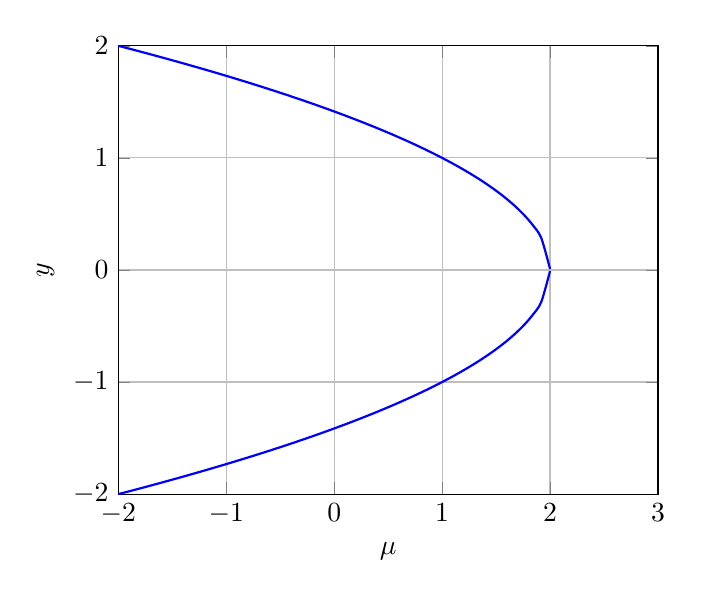
\begin{tikzpicture}
	\begin{axis}[
		smooth, no markers, grid,
		domain=-2:2,
		xmax=3, xmin=-2,
		ymax=2, ymin=-2,
		xlabel=$\mu $,
		ylabel=$y$]
		\addplot[thick, blue, samples=50]{sqrt(-x+2)};
		\addplot[thick, blue, samples=50]{-sqrt(-x+2)};
	\end{axis}
\end{tikzpicture}
\end{center}
Notice how for $\mu >2$, there are no equilibrium points, for $\mu =2$, there's 1, and for $\mu <2$, there's 2. Thus, $\mu =2$ is a \textbf{bifurcation} \textbf{value}.

However, bifurcations do not usually happen.
\begin{theorem}[Bifurcations]\label{thm:5}
	Let $\frac{\mathrm{d}y}{\mathrm{d}t} =f_\mu (y)$ be a one-parameter family. Then a bifrucation occurs  at $\mu =\mu _0$ if $f_{\mu _0}(y_0)=0$ and $f'_{\mu _0}(y_0)=0$.
\end{theorem}
\section{Linear Equations}
\begin{definition}[Linear Differential Equation]\label{dfn:8}
	A differential equation is called linear if it is linear in $y$ and it's derivatives. That is, every linear differential equation is of the form
	\[
		b(t)=\sum_{i=0}^{n} a_i(t)y^{(n)}(t)
	.\]
	We will generally study first order linear differential equations, which are of the form
	\[
		\frac{\mathrm{d}y}{\mathrm{d}t} =a(t)y + b(t)
	.\]
\end{definition}

In general, linear differential equations are not separable. However, they are simple to analyze analytically. Our methods for doing so vary based on the specific equation, so it's useful to precisely classify each equation.
\begin{definition}[Homogeneous]\label{dfn:9}
	Let
	\[
		\frac{\mathrm{d}y}{\mathrm{d}t} =a(t)y+b(t)
	.\]
	If $b(t)\equiv 0$ for all $t$, then we say the differential equation is \textbf{homogeneous}. If $b(t)$ is nonzero, we say the equation is nonhomogeneous.
\end{definition}

Linear differential equations act similarly to classic linear equations in many ways, and the next theorem formalizes some of these notions.
\begin{theorem}[Linearity]\label{thm:6}
	Let $\tilde{y}(t)$ solve the homogeneous equation
	\[
		\frac{\mathrm{d}y}{\mathrm{d}t} =a(t)y
	.\]
	Then any constant multiple $C\in\mathbb{R}$ of $\tilde{y}$ also solves the differential equation. That is,
	\[
		\frac{\mathrm{d}y}{\mathrm{d}t} =a(t)\tilde{y} \implies \frac{\mathrm{d}y}{\mathrm{d}t} =a(t)C\tilde{y}
	.\]

	Now consider the non-homogeneous equation
	\[
		\frac{\mathrm{d}y}{\mathrm{d}t} =a(t)y+b(t)
	.\]
	\begin{itemize}
		\item If $y_h$ solves the associated homogeneous equation $y'=a(t)y$, and $y_n$ is any solution to the nonhomogeneous equation, then $y_h+y_n$ solves the nonhomogeneous equation.
		\item If $y_1,y_2$ are two solutions to the nonhomogeneous equation, then $y_2-y_1$ solves the associated homogeneous equation.
	\end{itemize}
\end{theorem}

Solving homogeneous equations is fairly trivial, since they're separable by definition. Let
\[
	\frac{\mathrm{d}y}{\mathrm{d}t} =a(t)y
.\]
It follows that
\begin{align*}
	&\implies  \frac{1}{y}\frac{\mathrm{d}y}{\mathrm{d}t} =a(t)\\
	&\implies \int \frac{1}{y}\frac{\mathrm{d}y}{\mathrm{d}t}  \,\mathrm{d} t=\int a(t) \,\mathrm{d} t\\
	&\implies \ln y=A(t)+C\\
	&\implies y=Ce^{A(t)}
.\end{align*}

Solving nonhomogeneous equations is more difficult, and a precise analytical method will be given in the next section.
\section{Integrating Factors}
\begin{theorem}[Integrating Factors]\label{thm:7}
	Let
	\[
		\frac{\mathrm{d}y}{\mathrm{d}t} =a(t)y+b(t)
	.\]
	Then in principle, there always exists a solution $y(t)$ for the differential equation. Specifically,
	\[
		y(t)=\left( e^{\int -a(t) \,\mathrm{d} t} \right) ^{-1}\int e^{\int -a(t) \,\mathrm{d} t}b(t) \,\mathrm{d} t
	.\]
	From here, we can obviously account for an IVP.
\end{theorem}
\begin{proof}
\[
	\frac{\mathrm{d}y}{\mathrm{d}t} =a(t)y+b(t)
.\]
Let $A(t)$ be any antiderivative of $-a(t)$. It follows that
\[
	e^{A(t)}\frac{\mathrm{d}y}{\mathrm{d}t} =a(t)e^{A(t)}y+b(t)e^{A(t)}
.\]
Rearranging, we have
\[
	e^{A(t)}\frac{\mathrm{d}y}{\mathrm{d}t} -a(t)e^{A(t)}y=b(t)e^{A(t)}
.\]
Notice that by the product rule,
\[
	\frac{\mathrm{d}}{\mathrm{d}t} \left( e^{A(t)}y(t) \right) =e^{A(t)}y'(t)+A'(t)e^{A(t)}y=e^{A(t)}\frac{\mathrm{d}y}{\mathrm{d}t} -a(t)e^{A(t)}y
.\]
This is the same as the lefthand side. Thus,
\[
	\frac{\mathrm{d}}{\mathrm{d}t} \left( e^{A(t)}y(t) \right) =b(t)e^{A(t)}
.\]
Integrate both sides, it follows that
\[
	e^{A(t)}y(t)=\int e^{A(t)}b(t) \,\mathrm{d} t
.\]
Rearranging, we have
\[
	y(t)= \left( e^{A(t)} \right) \int e^{A(t)}b(t) \,\mathrm{d} t
.\]
\end{proof}
\chapter{First Order Systems}
